\documentclass[twoside]{romjist}
\usepackage[top=4.3cm, bottom=5.7cm, left = 3.74cm, right = 3.75cm]{geometry}
\usepackage{times}
\usepackage{authblk}
\usepackage{graphicx} 
\usepackage{amsmath}
\usepackage{amssymb}
\usepackage{amsthm}
\usepackage{cite}
\usepackage{graphicx}
\usepackage{epstopdf}
\usepackage{amssymb}
\usepackage{chemfig}
\usepackage{centernot} 
\usepackage[labelsep=space]{caption}
\usepackage{parskip}
\usepackage{placeins}
\graphicspath{ {./figures/} }

\begin{document}

	% the following 4 statements are for final print editing
    %do not modify them yourself
    \issuevolume{X}%set volume
    \issuenumber{X}%set number
    \issueyear{XXXX}%set year
    \issuepages{XXX--XXX}%set pages
	
	\headauthors{Andrei George-Andrei}%short author string, for placement in heading
    \headtitle{Dynamic (run-time) partial reconfiguration of FPGAs}%short title string, for placement in heading
    
    % Article top matter (title, authors)
    \title{Dynamic (run-time) partial reconfiguration of FPGAs}%full title string
	
	\author{Andrei George-Andrei}%set name of author
	
	\affil{Faculty of Electronics, Telecommunications and Information Technology}%set name of faculty
	\affil{(Advanced Computing in Embedded Systems Master Program)}%set name of master program
	\affil{University POLITEHNICA of Bucharest}%set name of college
	\affil{{\small (Splaiul Independentei 313, Bucharest, Romania, 060042)}}
	\affil{{\small andrei.geoorge@gmail.com}}
	
	\affil{February 2022}%\date won't work
		
	% always issue maketitle before abstract
    \maketitle
	
	\begin{abstract}
	This paper will describe the state of the art of the area of partial reconfiguration
	computing. In the last years, the Field Programable Gate Array has encountered
	an exponential growth of interest. From using the FPGAs only for Application
	Specific Integrated Circuits (ASIC) design and validation, now the trend is to
	use the FPGA directly in the final product as a standalone computing unit. The
	advantage of this practice is that the ASIC design, validation and manufacturing
	time and costs will be drastically reduced or even disappear, because the time-
	on-the-market of the product has the highest priority. State of the art FPGAs
	have evolved from simple gate arrays to complex systems with high speeds that
	competes with the classical microcontrollers (MCU), that include embedded
	memory, digital signal processing units (DSP), clock multipliers made of phase
	lock loops (PLL), tens of thousands of look up tables (LUT) and even
	microprocessors. These days, the FPGAs come along with different
	reconfiguration options. The most challenging of them is the partial run-time
	reconfiguration. This technique gives the system the versatility to update its
	hardware configuration on-the-fly, after the device has booted and started
	running. Also called Dynamic Partial Reconfiguration, it will provide the system
	with the ability to parallelize its resources and will gain a software-like ability
	to perform scheduled tasks, but this time by rearranging its hardware by the
	program demand. This will be accomplished without any performance
	reduction. Important areas of Dynamic Partial Reconfiguration interest can be
	the ones like runtime adaptive super-computing, fault tolerant systems, adaptive
	embedded software accelerators, self-reconfigurable and self-arrangeable
	systems.
	\end{abstract}

	\section{Introduction}
	\hspace{0.5cm}
	Traditionally, Application Specific Integrated Circuits (ASICs) are preferred for the final
	product. The prototyping and testing of the ASICs is accomplished by the help of Field
	Programable Gate Array devices. The ASICs are the best choice for the mass production
	processes, because the cost of the production masks is being amortized by the large number of
	sold units. The last trend, on the other side, when speaking of low serial production, the Field
	Programable Gate Arrays are preferred. This is because the development time is reduced, and
	the greatest part of the production price is reduced by eliminating the need of the production
	masks. These being said, the FPGAs are the best choice when talking about a low serial
	production and custom designs, because of their hardware versatility and ability to emulate
	almost every existing digital circuit. The Field Programable Gate Arrays also come with a
	series of advantages, like high computing speeds, capable memory blocks, Digital Signal
	Processing units and even microprocessors. Also, the existence of the Intellectual Property (IP)
	Cores offered by the vendors are drastically reducing the time and costs of development of the
	final product \cite{1} \cite{9}.
	One major feature of the FPGAs that this paper will be discussing is the Partial Reconfiguration
	ability. This is the ability of the FPGA to change its hardware component structure at the run
	time. One advantage could be the parallelization of the tasks in a system. Let’s consider a pure
	software system running on a Real Time Operating System (RTOS): all the hardware resources
	(Random Access Memory, processors, communications, peripherals, etc.) are already allocated
	and the configuration will remain the same for the whole operation time. Let’s further assume
	that one of the subsystems will crash, resulting in the partial or total system failure. A dynamic
	partial reconfigurable FPGA-based system can be a better implementation of the earlier
	example. The main advantage of the run-time reconfigurable system is that while it is running
	it can easily change its hardware configuration, replacing pieces of subsystems or
	implementing them in different regions of the FPGA. Another advantage of this kind of system
	could be that in comparison with the RTOS tasks, the reconfigurable system can allocate or
	deallocate hardware subsystems in such way that only when they will be needed (for example
	as a periodic or sporadic task) they will be implemented in the circuit (they will be allocated
	when their functionality is needed and when they finish their job, they will be deallocated,
	erased from the hardware, and another circuit for another task can replace them). When the
	hardware resources are limited, or some low power requirements must be accomplished or
	even if the system is running in harsh (ex: radiation) \cite{8} environment that can damage certain
	subsystems or subsystems parts, the Dynamic Partial Reconfiguration Systems can be the best
	choice. These reconfigurable can provide a high advantage in terms of power saving, task
	parallelization or even self-recovery when talking about fault tolerant systems \cite{2}.
	
	\section{Reconfiguration Techniques and Systems}
	\hspace{0.5cm}
	In order to better understand the concept of Partial Reconfiguration (PR), the following terms
	must be discussed: granularity, reconfiguration rate, system coupling and types of
	reconfiguration techniques. System data transfer, latency, power consumption, throughput and
	overhead are some parameters influenced by the above properties \cite{1} \cite{2}.
	
	\subsection{Reconfiguration Techniques}
	\hspace{0.5cm}
	FPGAs are configured with a sequence of bits called bitstream. In the past, the FPGAs were
	configured with a single static bitstream as a full configured system. On the other hand, on
	these days the vendors offer some reconfiguration techniques that allow us to perform partial
	or full reconfiguration of the FPGA bitstream \cite{1}:
	\begin{itemize}
		\item
		\textbf{Full Reconfiguration:} also known as total or global reconfiguration, this device
		programming method is a dynamic full reconfiguration that allows the configuration of
		the entire device without the need to reboot the external circuitry.
		
		The main advantage is that this type of reconfiguration is supported by most of the
		FPGAs available on the market.
		
		The disadvantage, although is that the bitstreams have large sizes (because the whole
		configuration is replaced). The consequences of the large bitstream sizes are that the
		reconfiguration time will be long (seconds), when reconfiguring, the power
		consumption will increase, and the storage demands will increase. The main
		disadvantage is that the whole system will be suspended while the reconfiguration is
		being done.
		\item
		\textbf{Partial Reconfiguration:} this type of reconfiguration allows to modify only on portion
		of the FPGA. A simple concept can be seen in Figure \ref{fig:figure21}.
		
		\begin{figure}[h]
			\centering
			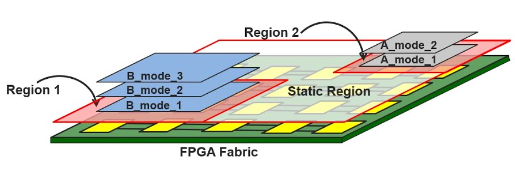
\includegraphics[width=\textwidth]{fig_2_1}
			\caption{Partial Reconfiguration Concept \cite{4}}
			\label{fig:figure21}
		\end{figure}
		
		Furthermore, this type can be classified into two subcategories:
		\begin{itemize}
			\item
			\textbf{Non-disruptive (runtime or dynamic):} this type implies that the parts that are
			not being replaced will remain operational at the run-time. The advantage of
			this method is the reduced reconfiguration time ranging from milliseconds to a
			few seconds.
			\item
			\textbf{Disruptive (non-dynamic):} when this partial reconfiguration technique is
			applied, the rest of the system will be affected due to the clock dependencies
			that will hold the clock or input/output ports dependencies where the ports must
			be kept in high impedance. The advantage of this technique is reduced memory
			required for bitstreams and less power consumption.
		\end{itemize}
		(The main disadvantages for both disruptive and non-disruptive Partial
		Reconfiguration techniques are the lack of tools and design software available, or
		when available, the complexity of the tools.)
		\item
		\textbf{Self-Reconfiguration:} it is referred as a separate technique, although it is a partial
		reconfiguration one. In this technique, the FPGA will control its own reconfiguration
		process and have its own decisions. It is a more complex type of partial reconfiguration,
		usually augmented by artificial intelligence algorithms \cite{7}.
	\end{itemize}
	\hspace{0.5cm}
	In the figure above (Figure \ref{fig:figure21}) \cite{4}, we can see a simple concept on how the Partial
	Reconfiguration is working. On the FPGA mapping we can see two types of regions:
	\begin{itemize}
		\item
		Static region (transparent white)
		\item
		Dynamic region (transparent red)
	\end{itemize}
	\hspace{0.5cm}
	The static region is the part of the FPGA where the bitstream will not change the whole
	program life. On the other hand, the red portions are called dynamic regions. These are the
	regions where the partial reconfiguration takes place. We can see for the Region 1 that
	several bitstreams can be loaded (Bmode1, Bmode2, Bmode3) and for the Region
	2 Amode1 and Amode2 bitstreams can be loaded, resulting in total of six possible
	combinations for the configuration \cite{4}.
	
	\subsection{Granularity}
	\hspace{0.5cm}
	When talking about partial reconfiguration, an important property of the system is the
	granularity \cite{1}. This is defined as the smallest function that can be replaced (modified) in the
	design. This can be classified into three types:
	\begin{itemize}
		\item
		Coarse granularity: complete IP cores are modified (reconfigured)
		\item
		Medium granularity: only parts of IP cores are reconfigured (register level)
		\item
		Low granularity: single or several bits are modified
	\end{itemize}
	\hspace{0.5cm}
	Low granularity offers the system high versatility, but at the same time it will increase the
	reconfiguration time. On the other hand, coarse granularity will speed-up the reconfiguration
	time, but the system will lower its flexibility.
	
	\subsection{System coupling types}
	\hspace{0.5cm}
	Usually, a reconfigurable system consists in a microprocessor and a reconfigurable device
	(FPGA reconfigurable material). The microprocessor must run the basic tasks, peripherals
	control, or the operating system, while the FPGA will take care of the high resource demanding
	tasks, this way an optimum parallelism is achieved. In Figure \ref{fig:figure22} we can see several coupling
	schemes \cite{3}.
	
	A more detailed classification of the coupling schemes can be seen below \cite{3}:
	\begin{itemize}
		\item
		\textbf{External stand-alone:} the reconfigurable hardware is connected to the microprocessor
		inputs and outputs, and it is fully independent. The microprocessor is the host, and the
		FPGA is the functional unit tied to the main microprocessor data receiver.
		\item
		\textbf{Attached processing unit:} in this case, the microprocessor is the host, and the FPGA
		is a coprocessor unit. Both of them are independent and the FPGA is used for leveraging
		heavy computing tasks off the microprocessor. The FPGA does not need the
		supervision of the microprocessor.
		\item
		\textbf{Coprocessor:} between the first two types. The reconfigurable fabric is located in the
		data cache, and it can be used either as cache resource or as computing resource.
		\item
		\textbf{Reconfigurable functional unit:} it permits to define custom instructions as a part of the
		microprocessor unit.
		\item
		\textbf{Microprocessor embedded in the FPGA fabric:} the microprocessor can be a
		hardware core that is burned definitely in the FPGA (cannot be reconfigured) or either
		a soft processor core that can be replaced by reconfiguring that region before run-time
		(static region).
	\end{itemize}

	\begin{figure}[h]
		\centering
		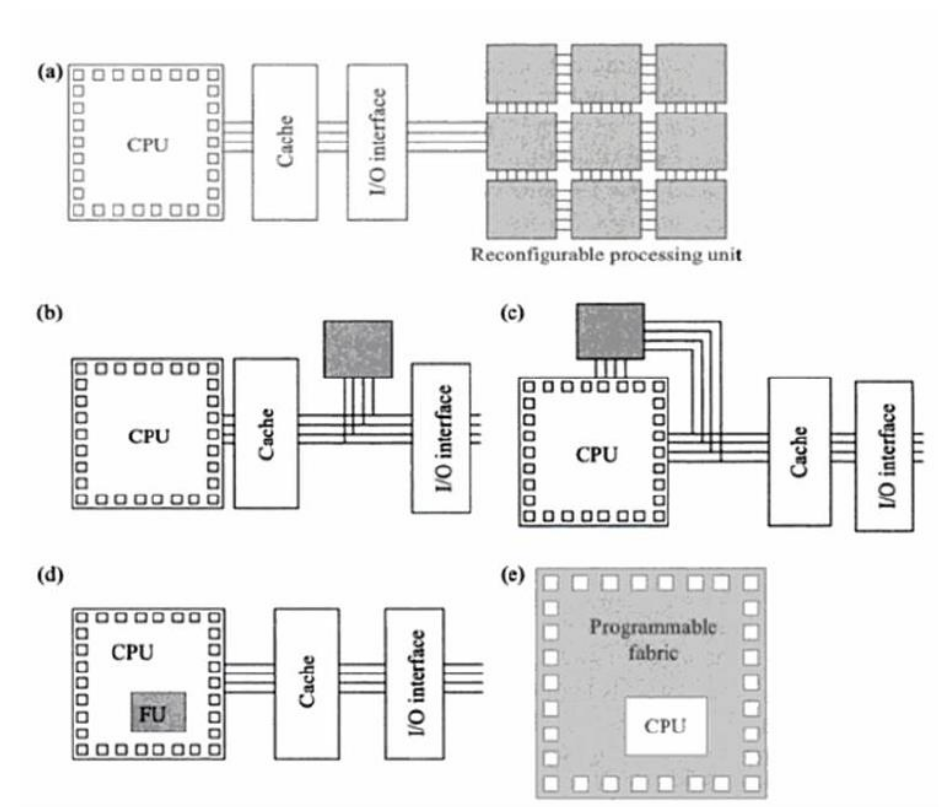
\includegraphics[width=\textwidth]{fig_2_2}
		\caption{Coupling Schemes \cite{3}}
		\label{fig:figure22}
	\end{figure}
	
	\subsection{Reconfiguration rate of system}
	\hspace{0.5cm}
	This parameter defines how often the system must be reconfigured \cite{1}. There are three main
	reconfiguration rate classes \cite{7}:
	\begin{itemize}
		\item
		\textbf{Context-switch:} reconfiguration occurs in order to change some parts of the system, or
		to change the context of the operating system. This is done at a very low rate, meaning
		once a day, month, or even year. Because of this, the reconfiguration delays are not
		important.
		\item
		\textbf{Runtime:} the reconfiguration is done at the beginning of a task while the other tasks
		are still running in parallel (multi-context) or even when the system does not have any
		tasks defined (single-context). It requires a low reconfiguration rate, and it must not
		affect the system or other running tasks integrity.
		\item
		\textbf{Realtime:} at the runtime, the reconfiguration time must be precise, and the process must
		be transparent. Also, the reconfiguration must be masked (all other tasks dependent on
		the reconfigurable fabric must not be running). For the moment, this type is not strongly
		supported, but its complexity could make it very precise in real-time applications.
	\end{itemize}
	
	\section{Architectures}
	\hspace{0.5cm}
	Effective logic capacity increasing and reconfiguration time reducing are the main desired
	topics when talking about Dynamic Partial Reconfiguration. In the early years, the major
	constrains of implementing large designs were the limited resource available in the FPGA and
	the slow reconfiguration caused by fetching big configuration files \cite{2} \cite{9}.
	
	\begin{figure}[h]
		\centering
		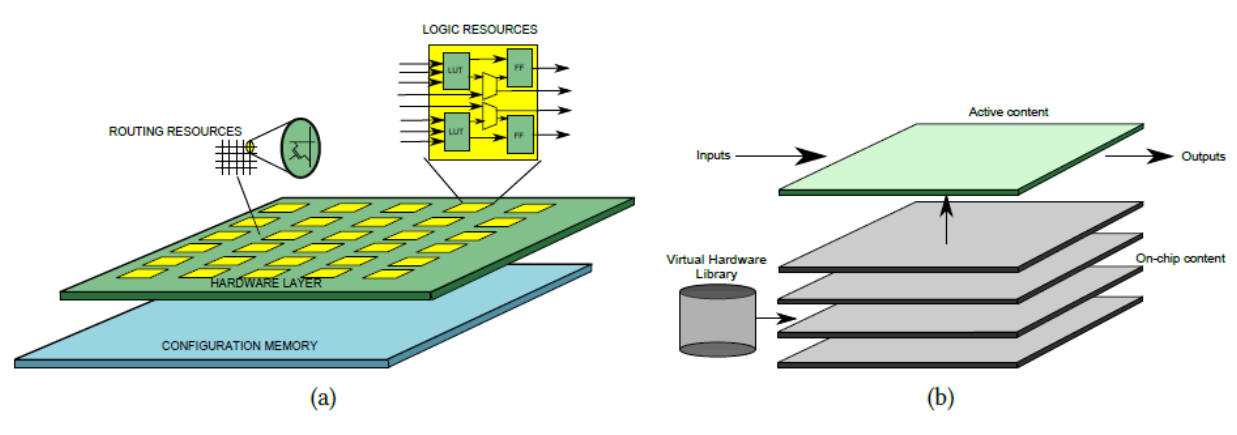
\includegraphics[width=\textwidth]{fig_3_1}
		\caption{a) Typical FPGA architecture. b) Multi-context FPGA architecture with several
		configuration memory layers \cite{2}}
		\label{fig:figure31}
	\end{figure}
	
	\hspace{0.5cm}In the above Figure \ref{fig:figure31} b) we see how the early dynamic reconfiguration architectures dealt
	with these limitations by increasing the number of configuration context layers. The last
	generation FPGAs does not lack of hardware resources. In the early days, the partial
	reconfiguration was used due to lack of resources, but now its target is, for example, to keep
	alive communications during system reconfiguration, or even sharing the reconfigurable
	resources between multiple users.
	
	\subsection{Academic and non-commercial architectures}
	\hspace{0.5cm}
	The first dynamic reconfiguration system was filled by Xilinx in 1995 as a patent for an FPGA
	that can store several configurations at the same time. In the first design, two configuration
	memory arrays were available in the FPGA, and they could store different configuration
	bitstreams. This idea was enhanced in 1997 with a time multiplexed FPGA based on the Xilinx
	XC4000E product.
	
	\textbf{\newline GARP architecture}
	
	\hspace{0.5cm}It was a dynamic reconfiguration architecture based on a standard MIPS processor combined
	with reconfigurable hardware \cite{2}.
	
	\hspace{0.5cm}The reconfigurable hardware was used as a slave, and it was placed on the same configuration
	layer with the microprocessor, as seen in Figure \ref{fig:figure32} a.
	
	\hspace{0.5cm}The program running on the processor oversaw loading and executing the reconfiguration from
	the configuration array. Also, the reconfigurable fabric had access to the standard memory
	hierarchy of the processor. Each reconfigurable array was divided into blocks. One block was
	used for control and the others for logic operations.
	
	\hspace{0.5cm}The architecture used partial array configuration as individual blocks.
	
	\begin{figure}[h]
		\centering
		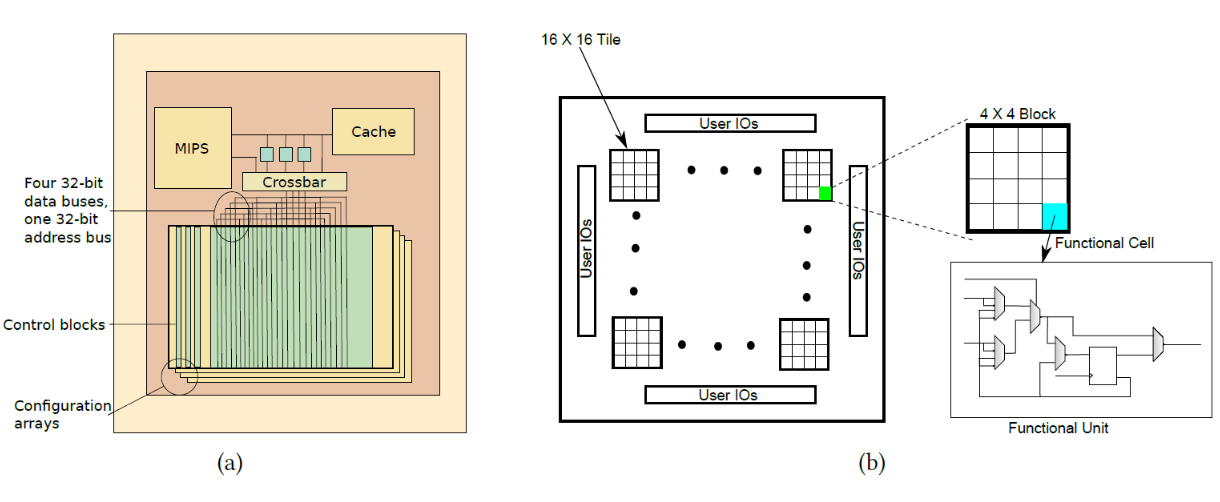
\includegraphics[width=\textwidth]{fig_3_2}
		\caption{a) GARP architecture. b) Xilinx XC6200 architecture \cite{2}}
		\label{fig:figure32}
	\end{figure}
	
	\subsection{Commercial Devices supporting Partial Reconfiguration}
	\hspace{0.5cm}
	In the present, only Xilinx and Altera are supporting Partial Reconfiguration architectures \cite{2}.
	We will only focus on the Xilinx FPGAs.
	
	\textbf{\newline Xilinx FPGAs}
	
	\hspace{0.5cm}Xilinx had supported Partial Reconfiguration for two decades, so they are the most popular
	manufacturers when talking about this kind of applications \cite{7}.
	
	
	\hspace{0.5cm}The first Partial Reconfiguration FPGA developed by Xilinx was the XC6200 series seen in
	Figure \ref{fig:figure32} b. This contained only one configuration memory layer and the architecture was
	divided into functional cells found inside divided tiles-like memory regions. The functional
	cells contained multiplexers for combinational logic, and routing resources.
	
	
	\hspace{0.5cm}The Virtex-II and Virtex-II Pro family made the Partial Reconfiguration more popular. In this
	architecture, the reconfigurable fabric was arranged in column fashion. These FPGA column
	primitives contains configurable logic clocks (CLBs), Block RAMs (BRAMs) and multipliers.
	The CLBs are made of look up-tables (LUTs) and Flip-Flops in two slices \cite{5}.
	
	
	\hspace{0.5cm}ICAP (Internal Configuration access Port) has been introduced by the Virtex devices family.
	The ICAP has been a major step, because it allows the FPGA fabric to load partial bitstreams.
	The bitstreams can be fetched from outside of the FPGA fabric with the help of a soft-processor
	or a custom state machine that is already loaded and running onto the FPGA fabric. This will
	result in a circuit implementation that can modify itself \cite{5}.
	
	
	\hspace{0.5cm}The latest Xilinx FPGAs supporting Dynamic Partial Reconfiguration are the Virtex-5 and
	Zinq-7000 device families. Both architectures can be seen in Figure \ref{fig:figure33} \cite{5}.
	
	
	\begin{figure}[h]
		\centering
		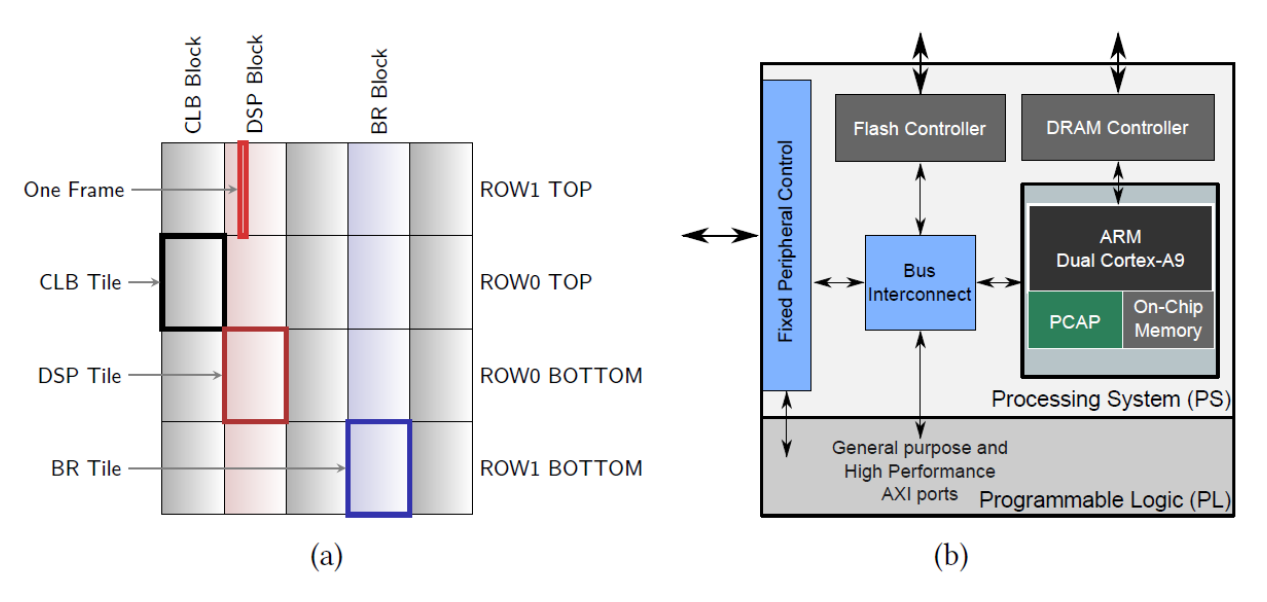
\includegraphics[width=\textwidth]{fig_3_3}
		\caption{a) Xilinx Virtex architecture. b) Zynq SoC architecture \cite{5}}
		\label{fig:figure33}
	\end{figure}
	
	\section{Development tools for Partial Reconfiguration}
	\hspace{0.5cm}
	The main FPGA manufacturers that support Partial Reconfiguration are Xilinx and Altera.
	They also offer support for the development of Partial Reconfiguration synthetization. In the
	table below \cite{2} (Figure \ref{fig:figure41}) we can see the main features of Xilinx, Altera and other vendors
	for the software that they are offering for Partial Reconfiguration \cite{2} \cite{6}.
	
	
	\hspace{0.5cm}A white dot means that operation is fully manual or not supported, a black and white dot means
	partial automation or support provided by the tool and a full black dot means that the step is
	fully automated by the tool requiring no designer intervention.
	
	\begin{figure}[!htbp]
		\centering
		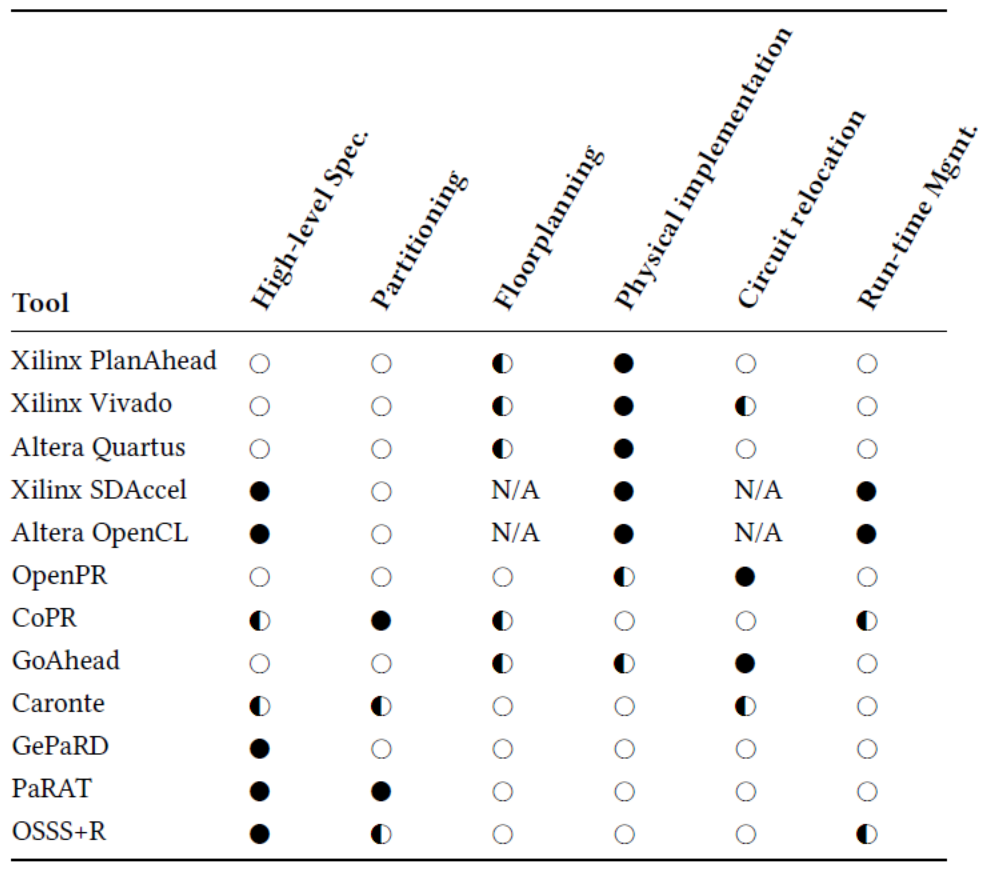
\includegraphics[width=\textwidth]{fig_4_1}
		\caption{Comparison features supported by different PR tools \cite{2}}
		\label{fig:figure41}
	\end{figure}
	\FloatBarrier
	
	\section{Conclusion and further work}
	\hspace{0.5cm}In the last years, the ASIC world has been surpassed by the FPGAs in the custom hardware
	and low mass production field. The need of fast developing computing intensive embedded
	devices has led to a progress increase in the FPGA research and development.
	
	
	\hspace{0.5cm}The Dynamic (run-time) Partial Reconfiguration on FPGAs topic was opened in 1995 because
	of the lack of hardware resource on the reconfigurable fabric, but these days this topic is
	growing fueled by other necessities, like the need to share the same resource with multiple
	users, switch hungry tasks by rearranging parts of the hardware subsystems in multitasking,
	save power by disabling subsystems, creating self-recovering systems that can rebuild its own
	subsystems or even for fault tolerant systems that needs extra protection.
	
	
	\hspace{0.5cm}In conclusion, the Dynamic Partial Reconfiguration on FPGAs is a promising field that can
	accomplish hungry computing tasks withing a low power consumption that need to be further
	studied.

	\begin{thebibliography}{9}
	\bibliographystyle{plain}
	
	\bibitem{1} Y.E. Krasteva. Reconfigurable Computing Based on Commercial FPGAs. Solutions for
	the Design and Implementation of Partially Reconfigurable Systems, 2009
	
	\bibitem{2} KIZHEPPATT VIPIN and SUHAIB A. FAHMY. 2017. FPGA Dynamic and Partial
	Reconfiguration: A Survey of Architectures, Methods, and Applications. ACM Comput. Surv. 1,
	1, Article 1 (January 2017)
	
	\bibitem{3} Bashir Al-Hashimi. System-on-chip: Next Generation Electronics. IEE, 2006
	
	\bibitem{4} KIZHEPPATT VIPIN, Partial reconfiguration (youtube tutorial series) 2020
	
	\bibitem{5} Vivado Design Suite User Guide Partial Reconfiguration - UG909 (v2018.1), 2018
	
	\bibitem{6} Fernando Moraes, DYNAMIC AND PARTIAL RECONFIGURATION IN FPGA
	SOCS: REQUIREMENTS TOOLS AND A CASE STUDY
	
	\bibitem{7} Oswald Berthold, Self-reconfiguring System-on-Chip using Linux
	on a Virtex-5 FPGA, 2012
	
	\bibitem{8} Rashad S. Oreifej, A Sustainable Autonomic Architecture for Organically Reconfigurable
	Computing Systems, 2011
	
	\bibitem{9} Ahmed Al-Wattar, Efficient Scheduling,Mapping and Resource Prediction for Dynamic
	Run time Operating Systems, 2015
	
	\end{thebibliography}
	
\end{document}